\documentclass{beamer}
%
% Choose how your presentation looks.
%
% For more themes, color themes and font themes, see:
% http://deic.uab.es/~iblanes/beamer_gallery/index_by_theme.html
%
\mode<presentation>
{
  \usetheme{Szeged}      % or try Darmstadt, Madrid, Warsaw, ...
  \usecolortheme{beaver} % or try albatross, beaver, crane, ...
  \usefonttheme{professionalfonts}  % or try serif, structurebold, ...
  \setbeamertemplate{navigation symbols}{}
  \setbeamertemplate{caption}[numbered]
} 

\usepackage{cmap}
\usepackage[english,russian]{babel}
\usepackage[utf8x]{inputenc}
\usepackage{graphicx}
\usepackage{hyperref}
\usepackage{svg}
\usepackage{amsmath}
\usepackage{booktabs}
\usepackage{algorithm}
\usepackage{algpseudocode}
\usepackage{hyperref}
\usepackage{tikz}
\usetikzlibrary{arrows,shapes}
\usepackage{multicol}
\usepackage{lipsum}
\usepackage{mwe}
\usepackage{floatrow}
\usepackage{subfig}
\usepackage{times}
\usepackage{textcomp}
\usepackage{smartdiagram}
\usepackage{caption}
\usesmartdiagramlibrary{additions}
\usepackage[colorinlistoftodos]{todonotes}
\usepackage{wrapfig}
\usepackage{subcaption}
\captionsetup{compatibility=false}

\everymath{\displaystyle}
\DeclareMathOperator*{\argmin}{arg\,min}
\DeclareMathOperator*{\argmax}{arg\,max}


\title[Обучения с подкреплением]{Методы обучения с подкреплением для решения задач сборки}
\author{Юнес Али}
\institute[МГТУ им. Баумана]
{
  Рукаводитель: Ющенко \textsc{А.~С.}\\
  Московский Государственный Технический Университет имени Н.Э.Баумана 
}
\titlegraphic{%
  \begin{picture}(0,0)
    \put(25,40){\makebox(0,0)[rt]{
\includegraphics[width=2cm]{img/logo.png}}}
  \end{picture}}
\begin{document}
\date{}
\begin{frame}
  \titlepage
\end{frame}

% Uncomment these lines for an automatically generated outline.
\begin{frame}{Содержание}
  \tableofcontents
\end{frame}

\section{Введение}
\subsection{классическое управление робототехники}
\begin{frame}{классическое управление робототехники}
\begin{center}
\smartdiagramset{
uniform color list=gray!60!blue!20 for all items,
text width=5cm,
back arrow disabled=true,
module y sep=1.3cm
}
\smartdiagram[flow diagram:vertical]{наблюдение,оценка состояния,планирование движения,низкий уровень контроля,команды мотора}
\end{center}
\end{frame}
\subsection{глубокое обучение робототехники}
\begin{frame}
  \frametitle{глубокое обучение робототехники}
\begin{figure}[h]
    \centering
    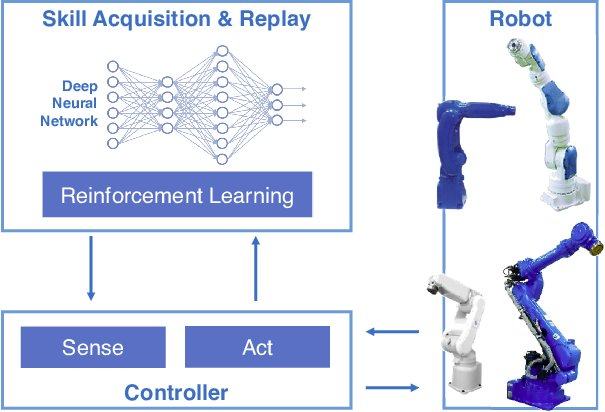
\includegraphics[width=6cm]{img/Rl-robot.jpg}
    \captionsetup{labelformat=empty}
    \caption{структура системы обучения}
\end{figure}
\end{frame}
\subsection{Постановка задачи}
\begin{frame}{Постановка задачи}
    \begin{itemize}
        \item "плотный зазор цилиндрический стержня в отверстии" \\ (Tight clearance cylindrical peg-in-hole task).
    \end{itemize}
    \begin{figure}[h]%
    \centering
    \subfloat[]{{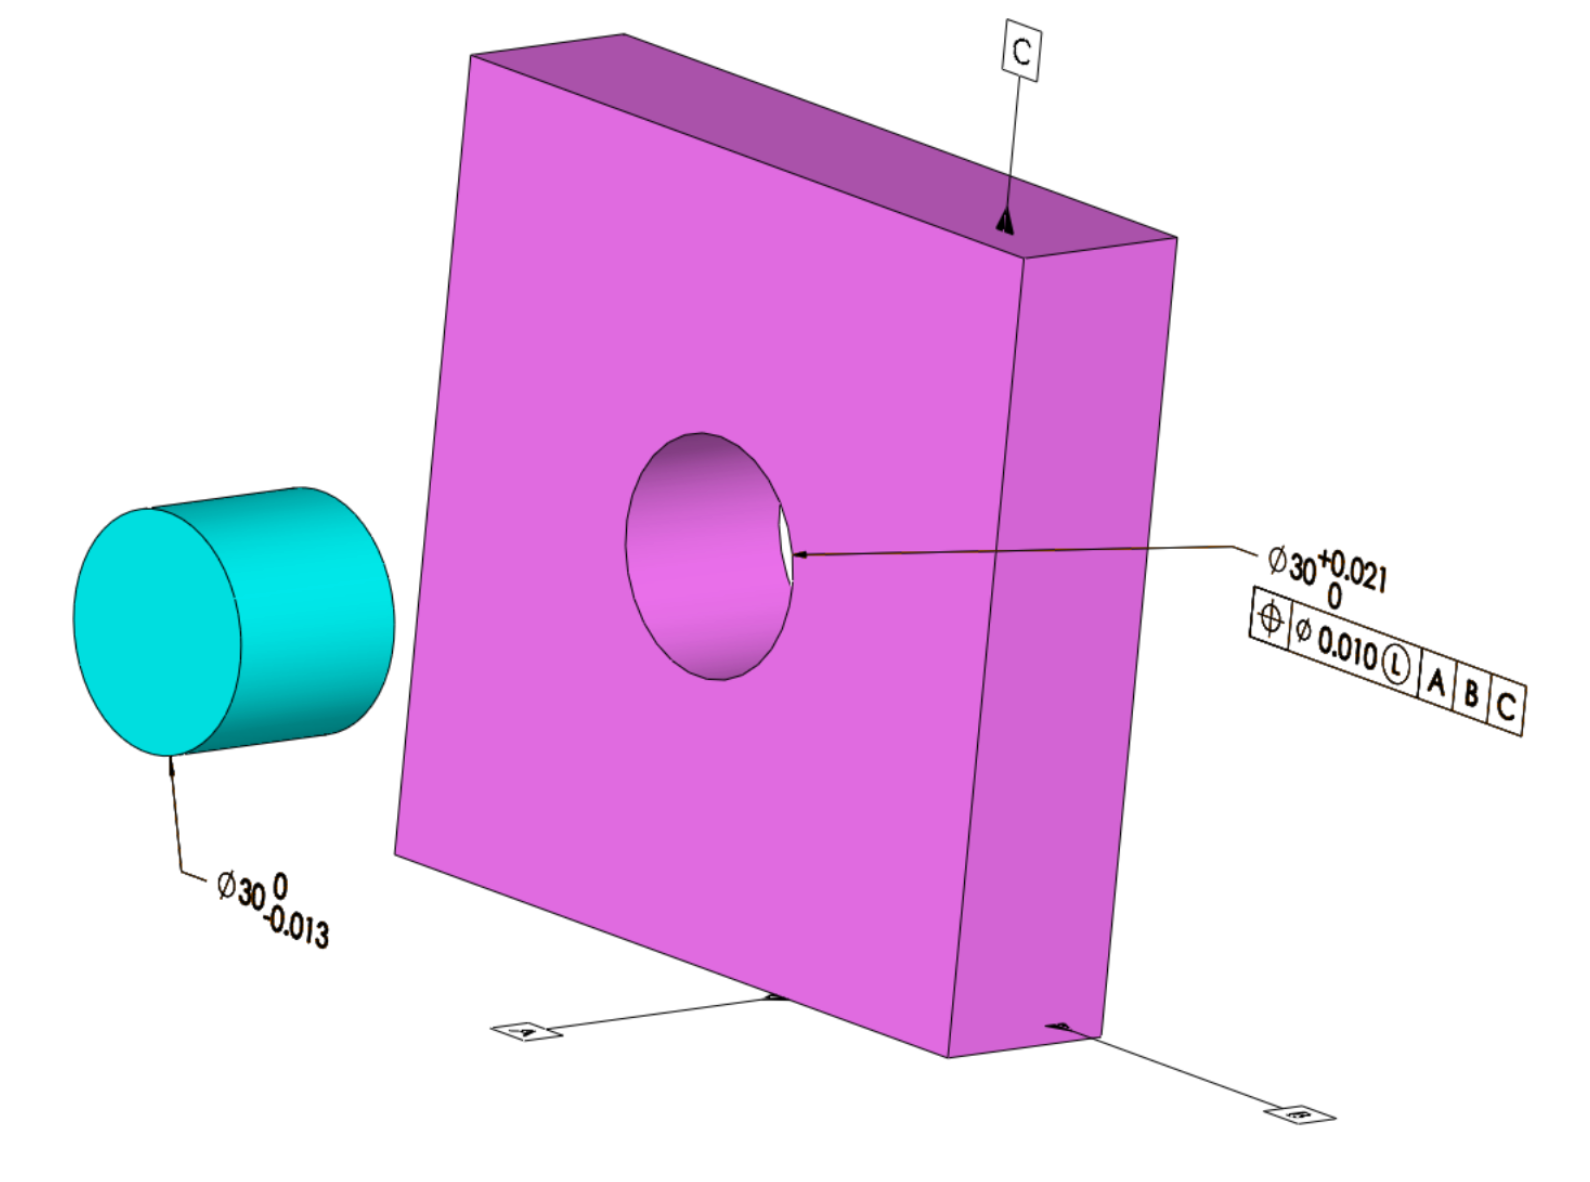
\includegraphics[width=4.5cm]{img/LMC.png} }}%
    \qquad
    \subfloat[]{{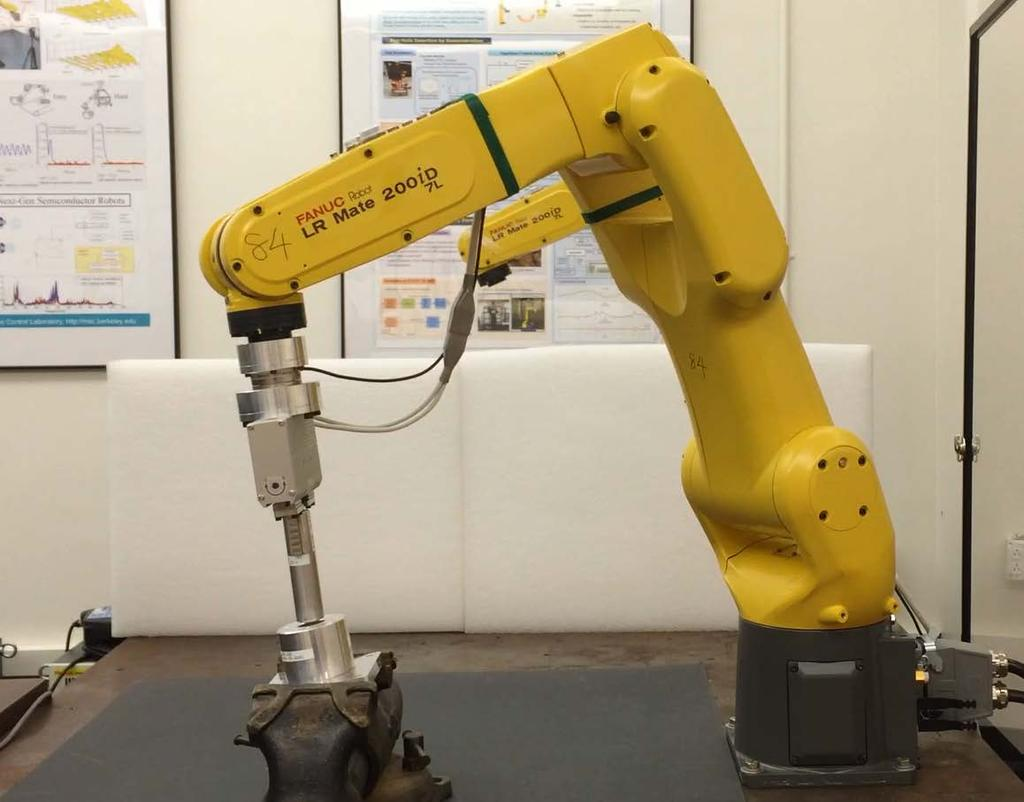
\includegraphics[width=4.5cm]{img/5-0.jpg} }}%
    \end{figure}
\end{frame}

\begin{frame}{Важность реализации проекта}
    \begin{itemize}
        \item Не зависит от модель робота (с точки зрения алгоритма динамеческий модель неизвесн)
        \item Необходимая Точность для выполнения задачи, превышает точность робота
        \item Сверхточные датчикы силы и момента  $\rightarrow $ камеру и датчики силы и положения
        \item Первый шаг к разработке \textbf{интеллектуального Робота }
    \end{itemize}
\end{frame}

\section{Направления исследований}
\subsection{Обучения с подкреплением}
\begin{frame}
  \frametitle{Обучения с подкреплением}
  \begin{itemize}
   \item Является подразделом машинного обучения, изучающим, как агент должен действовать в окружении, чтобы максимизировать некоторый долговременный выигрыш.
  \end{itemize}
  \begin{center}
 \captionsetup{labelformat=empty}
\captionof{figure}{Обучения с подкреплением}
    \tikzstyle{block} = [rectangle, draw, 
    text width=7em, text centered, rounded corners, minimum height=3em]
    \tikzstyle{line} = [draw, -latex]
    \begin{tikzpicture}[node distance = 6em, auto, thick]
        \node [block] (Agent) {Агент};
        \node [block, below of=Agent] (Environment) {Окружение};
        \path [line] (Agent.0) --++ (4em,0em) |- node [near start,align=center]{Действие \\ $a_t$} (Environment.0);
        \path [line] (Environment.180) --++ (-4em,0em) |- node [near start,align=center] {Cостояния \\ $s_{t+1}$ \\Награда \\$r_{t+1}$} (Agent.180);
    \end{tikzpicture}
\end{center}{}
\end{frame}

\begin{frame}{Обучения с подкреплением}
    \begin{center}
 \captionsetup{labelformat=empty}
\captionof{figure}{марковский процесс принятия решений}
 \begin{tikzpicture}[->, >=stealth', auto, thick, node distance=3cm]

    \tikzstyle{round}=[thick,draw=black,circle]

    \node[round] (s0) {$s_0$};
    \node[round,right= 25mm of s0] (s1) {$s_1$};
    \node[round,above right=7mm and 10mm of s0] (a1){$a_1$};
    \node[round,right= 25mm of s1] (s2) {$s_2$};
    \node[round,above right=7mm and 10mm of s1] (a2){$a_2$};
    \node[round,above right=7mm and 10mm of s2] (a3){$a_3$};

    \path (s0) edge node[below] {$p(s_{t+1}|s_t,a_t)$}(s1)
          (s0) edge node {$\pi_\theta$} (a1)
          (a1) edge node {} (s1);
    \path (s1) edge node[below] {$p(s_{t+1}|s_t,a_t)$}(s2)
          (s1) edge node {$\pi_\theta$} (a2)
          (a2) edge node {} (s2);
    \path (s2) edge node {$\pi_\theta$} (a3);
\end{tikzpicture}
\end{center}
\begin{itemize}
    \item $M={S,A,\tau,r}$
    \item Состояния : $s \in S$
    \item Действия : $a \in A$ , $a \sim \pi(a_t|s_t)$ 
    \item Вероятность переходов : $p(s_{t+1}|s_t,a_t)\in \tau $
    \item Функция вознаграждения : $ r : S \times A \to R $ 
\end{itemize}
\end{frame}

\subsection{Алгоритмы обучения с подкреплением}
\begin{frame}{Алгоритмы обучения с подкреплением}
    Самые важные современие адгоритмы \\ (без использования моделей):
\begin{enumerate}
    \item Алгоритмы с непрерывными моделями: DQN (2013), DDPG (2015)
    \item Алгоритмы градиента стратегии: TRPO (2015), \\ PPO (2017)
\end{enumerate}
\end{frame}

\begin{frame}{Алгоритмы обучения с подкреплением}
\begin{figure}
    \centering
    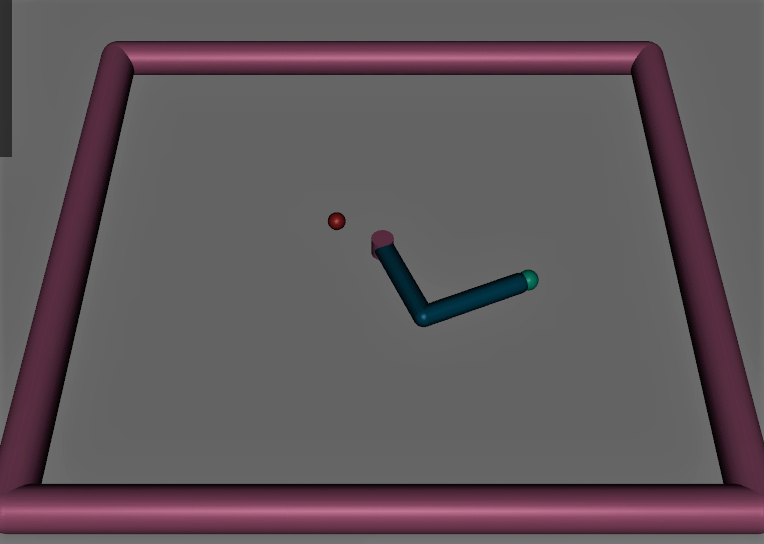
\includegraphics[width=7cm]{img/Reacher(Mujoco).png}
    \captionsetup{labelformat=empty}
    \caption{OpenAI gym environment "Reacher"}
\end{figure}

\end{frame}

\begin{frame}{Алгоритмы обучения с подкреплением}
\begin{center}
    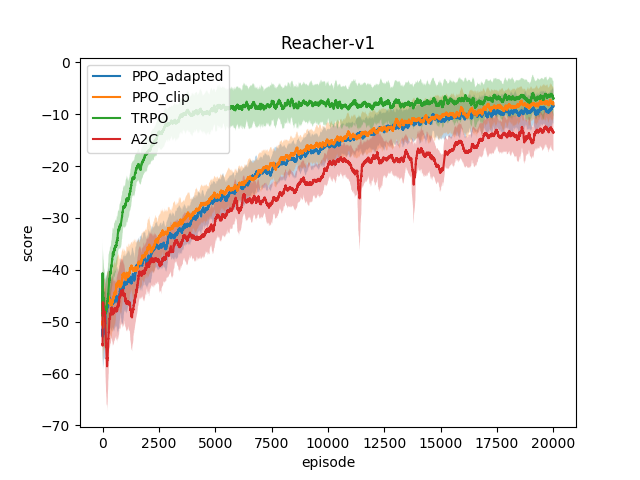
\includegraphics[width=9cm]{img/Reacher.png}
\end{center}
\end{frame}

\section{План работы}
\subsection{Новизна исследования}
\begin{frame}{Новизна исследования}
    \begin{itemize}
        \item В особом случае серийных роботов, мы можем направить робота использовать полезных образцов во время  процесса обучения.
        \item или мы используем гауссовские процессы, которые могут изучить модель среды из нескольких образцов.
        \item это направление исследований называется "Data-efficient reinforcement learning"
    \end{itemize}
\end{frame}
\subsection{Используемые технологии}
\begin{frame}{Используемые технологии}
    \begin{itemize}
        \item Python, Keras, Tensorflow
        \item KUKA LBR IIWA 14-r820
        \item ROS (Robotic Operatic System)
    \end{itemize}
\begin{figure}[h]
 
    \begin{subfigure}
        
\includegraphics[width=0.3\linewidth]{img/keras-tensorflow-logo.jpg} 
    \end{subfigure}
    \begin{subfigure}
        
\includegraphics[width=0.3\linewidth]{img/Ros_logo.png}
    \end{subfigure}
    \begin{subfigure}
        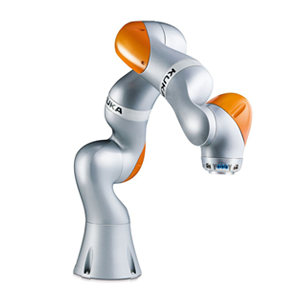
\includegraphics[width=0.2\linewidth]{img/iiwa.png}
    \end{subfigure}
\end{figure}
\end{frame}

\begin{frame}{План работы}
    \begin{enumerate}
        \item Следовать развития темы исследований (Научные статьи)
        \item Написать код алгоритмов (TRPO,PPO,DDPG)
        \item Подготовка робота и экспериментальной среды
        \item Попробовать алгоритм в симуляторе
        \item Попробовать алгоритм на реальном роботе
        \item Разработка алгоритма обучения
    \end{enumerate}
\end{frame}

\begin{frame}{Конец}
    \centering
    \Huge
    \emph{Спасибо за внимание!}
\end{frame}

\end{document}
